\subsection{Testing redshift dependence of luminosity correlations}
After reconstructing the redshift-distance modulus from the machine learning model, we can use it fit luminosity correlations. Luminosity correlations are connections between measurable parameters of the GRB vairables(light curves, spectra etc) with the GRB luminosity(L). The burst’s luminosity distance must be known to convert $P_{bolo}$ to $L$ (or $S_{bolo}$ to $E_{\gamma}$) and this is known only for bursts with measured redshifts.
\begin{align}
	\mu &= 5 \log \frac{d_{L}}{\mathrm{Mpc}}+25\\
	L &= 4 \pi d_{L}^{2} P_{\text {bolo }}
\end{align}
We are using the six luminosity correlations defined in \cite{schaefer2007hubble}.
\begin{enumerate}[noitemsep]
\item{Lag versus Luminosity ($T_{lag}-L$)}
\item{Variability versus Luminosity ($V-L$)}
\item{$E_{peak}$ versus Luminosity ($E_{peak}-L$)}
\item{$E_{peak}$ versus $E_{\gamma}$ ($E_{peak}-E_{\gamma}$)}
\item{$T_{RT}$ versus Luminosity ($T_{RT}-L$)}
\item{$E_{peak}$ versus $E_{iso}$ ($E_{peak}-E_{iso}$)}
\end{enumerate}
The observed luminosity indicators will have different values from those that would be observed in the rest frame of the GRB. That is, the light curves and spectra seen by Earth-orbiting satellites suffer time-dilation and redshift. The physical connection between the indicators and the luminosity is in the GRB rest frame, so we must take our observed indicators and correct them to the rest frame of the GRB.
\begin{align}
	T_{lag_i} &= \frac{T_{lag}}{1 + z}\\
	T_{RT_i} &= \frac{T_{RT}}{1 + z}\\
	V_i &= V(1 + z)\\
	E_{peak_i} &= E_{peak}(1 + z)
\end{align}
The calibration will essentially be a fit on a log-log plot of the luminosity indicator versus the luminosity. However, an important point is that the conversion from the observed redshift to a luminosity distance is independent of any cosmological model.
\begin{align}
\log \frac{L}{\operatorname{erg} \mathrm{s}^{-1}} &= a_{1}+b_{1} \log \frac{\tau_{\operatorname{lag}, i}}{0.1 s}, \\
\log \frac{L}{\operatorname{erg~s}^{-1}} &= a_{2}+b_{2} \log \frac{V_{i}}{0.02}, \\
 \log \frac{L}{\operatorname{erg~s}^{-1}} &= a_{3}+b_{3} \log \frac{E_{p, i}}{300 \mathrm{keV}}\\
\log \frac{E_{\gamma}}{\text { erg }} &= a_{4}+b_{4} \log \frac{E_{p, i}}{300 \mathrm{keV}}, \\
\log \frac{L}{\text { erg s }} &= a_{5}+b_{5} \log \frac{\tau_{\mathrm{RT}, i}}{0.1 \mathrm{~s}}, \\
\log \frac{E_{\text {iso }}}{\text { erg }} &= a_{6}+b_{6} \log \frac{E_{p, i}}{300 \mathrm{keV}}
\end{align}
Hence, the uncertainty of $L$ propagates from the uncertainties of $P_{\text {bolo }}$ and $d_{L}$. The isotropic equivalent energy $E_{\text {iso }}$ can be obtained from the bolometric fluence $S_{\text {bolo }}$ by
$$
E_{\text {iso }}=4 \pi d_{L}^{2} S_{\text {bolo }}(1+z)^{-1},
$$
the uncertainty of $E_{iso}$ propagates from the uncertainties of $S_{bolo}$ and $d_L$. If on the other hand, GRBs radiate in two symmetric beams, then we can define the collimation-corrected energy $E_{\gamma}$ as
$$
E_{\gamma} \equiv E_{\text {iso }} F_{\text {beam }},
$$

where $F_{\text {beam }} \equiv 1-\cos \theta_{\text {jet }}$ is the beaming factor, $\theta_{\text {jet }}$ is the jet opening angle. The uncertainty of $E_{\gamma}$ propagates from the uncertainties of $E_{\text {iso and }} F_{\text {beam }}$.

In order to test if the correlations discussed in the above section vary with redshift, we divide the GRB samples into two subsamples corresponding to the following redshift bins: the low-z sample ($z \leq 1.4$) which consists of 50 GRBs, and the high-z sample ($z > 1.4$) which consists of 66 GRBs. We investigate the redshift dependence of luminosity correlations for this two subsamples, as well as for the full GRBs sample. To fit the six luminosity correlations, we apply the D’Agostini’s liklihood\cite{d2005fits}
$$
\mathcal{L}\left(\sigma_{\mathrm{int}}, a, b\right) \propto \prod_{i} \frac{1}{\sqrt{\sigma_{\mathrm{int}}^{2}+\sigma_{y i}^{2}+b^{2} \sigma_{x i}^{2}}} \times \exp \left[-\frac{\left(y_{i}-a-b x_{i}\right)^{2}}{2\left(\sigma_{\mathrm{int}}^{2}+\sigma_{y i}^{2}+b^{2} \sigma_{x i}^{2}\right)}\right]
$$
For each correlation and each redshift bin, By maximizing this joint likelihood function, we can derive the best-fitting parameters $a$, $b$ and the intrinsic scatter $\sigma_{int}$, where the intrinsic scatter $\sigma_{int}$ denotes any other unknown errors except for the measurement errors. The results of the fits and the number of GRBs used in each fit are summarized in \eqref{table_pantheon_gp}.
\begin{table} [H]
\centering
\begin{tabular}{|c|c|c|c|c|c|c|c|c|}
\hline
Correlation & sample & N & a & $a_{err}$ & b & $b_{err}$ & $\sigma$ & $\sigma_{int}$\\
\hline
\multirow{3}{*}{$T_{lag}-L$} & low-z & 37 & 52.09 & 0.11 & -0.78 & 0.16 & 0.51 & 0.09\\
\cline{2-9}
 & high-z & 32 & 52.59 & 0.07 & -0.65 & 0.12 & 0.22 & 0.09\\
\cline{2-9}
 & All-z & 69 & 52.32 & 0.07 & -0.76 & 0.11 & 0.47 & 0.06\\
\hline
\multirow{3}{*}{$V-L$} & low-z & 47 & 52.1 & 0.25 & 0.65 & 0.37 & 0.93 & 0.14\\
\cline{2-9}
 & high-z & 57 & 52.8 & 0.15 & 0.34 & 0.14 & 0.62 & 0.07\\
\cline{2-9}
 & All-z & 104 & 52.38 & 0.14 & 0.6 & 0.15 & 0.76 & 0.07\\
\hline
\multirow{3}{*}{$E_{peak}-L$} & low-z & 50 & 51.87 & 0.09 & 1.47 & 0.19 & 0.59 & 0.07\\
\cline{2-9}
 & high-z & 66 & 52.48 & 0.06 & 1.15 & 0.15 & 0.3 & 0.06\\
\cline{2-9}
 & All-z & 116 & 52.17 & 0.06 & 1.44 & 0.14 & 0.55 & 0.05\\
\hline
\multirow{3}{*}{$E_{peak}-E_{\gamma}$} & low-z & 12 & 50.63 & 0.08 & 1.56 & 0.19 & 0.23 & 0.09\\
\cline{2-9}
 & high-z & 12 & 50.74 & 0.14 & 1.17 & 0.43 & 0.39 & 0.14\\
\cline{2-9}
 & All-z & 24 & 50.67 & 0.07 & 1.47 & 0.17 & 0.26 & 0.07\\
\hline
\multirow{3}{*}{$T_{RT}-L$} & low-z & 39 & 52.69 & 0.13 & -1.34 & 0.19 & 0.48 & 0.07\\
\cline{2-9}
 & high-z & 40 & 52.86 & 0.08 & -0.81 & 0.17 & 0.34 & 0.07\\
\cline{2-9}
 & All-z & 79 & 52.77 & 0.08 & -1.23 & 0.13 & 0.45 & 0.05\\
\hline
\multirow{3}{*}{$E_{peak}-E_{iso}$} & low-z & 40 & 52.56 & 0.1 & 1.6 & 0.2 & 0.6 & 0.08\\
\cline{2-9}
 & high-z & 61 & 53.0 & 0.06 & 1.27 & 0.14 & 0.38 & 0.04\\
\cline{2-9}
 & All-z & 101 & 52.8 & 0.06 & 1.53 & 0.13 & 0.52 & 0.04\\
\hline
\end{tabular}
\caption{Best fitting parameters for luminsoity correlations. N is the number of GRB samples.}
\label{table_pantheon_gp}
\end{table}

We perform a Markov Chain Monte Carlo analysis to calculate the posterior probability density function (PDF) of parameter space. We assume a flat prior on all the free parameters and limit $\sigma_{\text {int }}>0$. Note that not all GRBs can be used to analyze each luminosity correlation, because not all the necessary quantities are measurable for some GRBs. For example, GRBs without measurement of the spectrum lag can not used in the $\tau_{\text {lag }}-L$ analysis. Hence, we present the best-fitting parameters, together with the number of available GRBs in each fitting in Table \eqref{table_pantheon_gp} In Figure \eqref{fig:correlation_gp} we plot all the six luminosity correlations in logarithmic coordinates. Low-z and high-z GRBs are represented by blue and red dots with the error bars denoting $1 \sigma$ uncertainties. The blue line, red line and black line stand for the best-fitting results for low-z GRBs, high-z GRBs and all-z GRBs, respectively.

As shown in Table \eqref{table_pantheon_gp} low-z GRBs have a smaller intercept, but a sharper slope than high-z GRBs for all the six luminosity correlations. All-z GRBs have the parameter values between that of low-z and high-z subsamples. For the intrinsic scatter, low-z GRBs have larger value than high-z GRBs, and the $E_{p}-E_{\gamma}$ relation has the smallest intrinsic scatter hence we can only obtain its upper limit. The $V-L$ relation has the largest intrinsic scatter, thus it can not be fitted well with a simple line, which is legible in Figure \eqref{fig:correlation_gp}. $E_{p}-E_{\gamma}$ relation of low-z GRBs is consistent with that of high-z GRBs at $1 \sigma$ confidence level. For the rest luminosity correlations, however, the intercepts and slopes for low-z GRBs differ from that of high-z GRBs.

\begin{figure}[H]
	\centering
	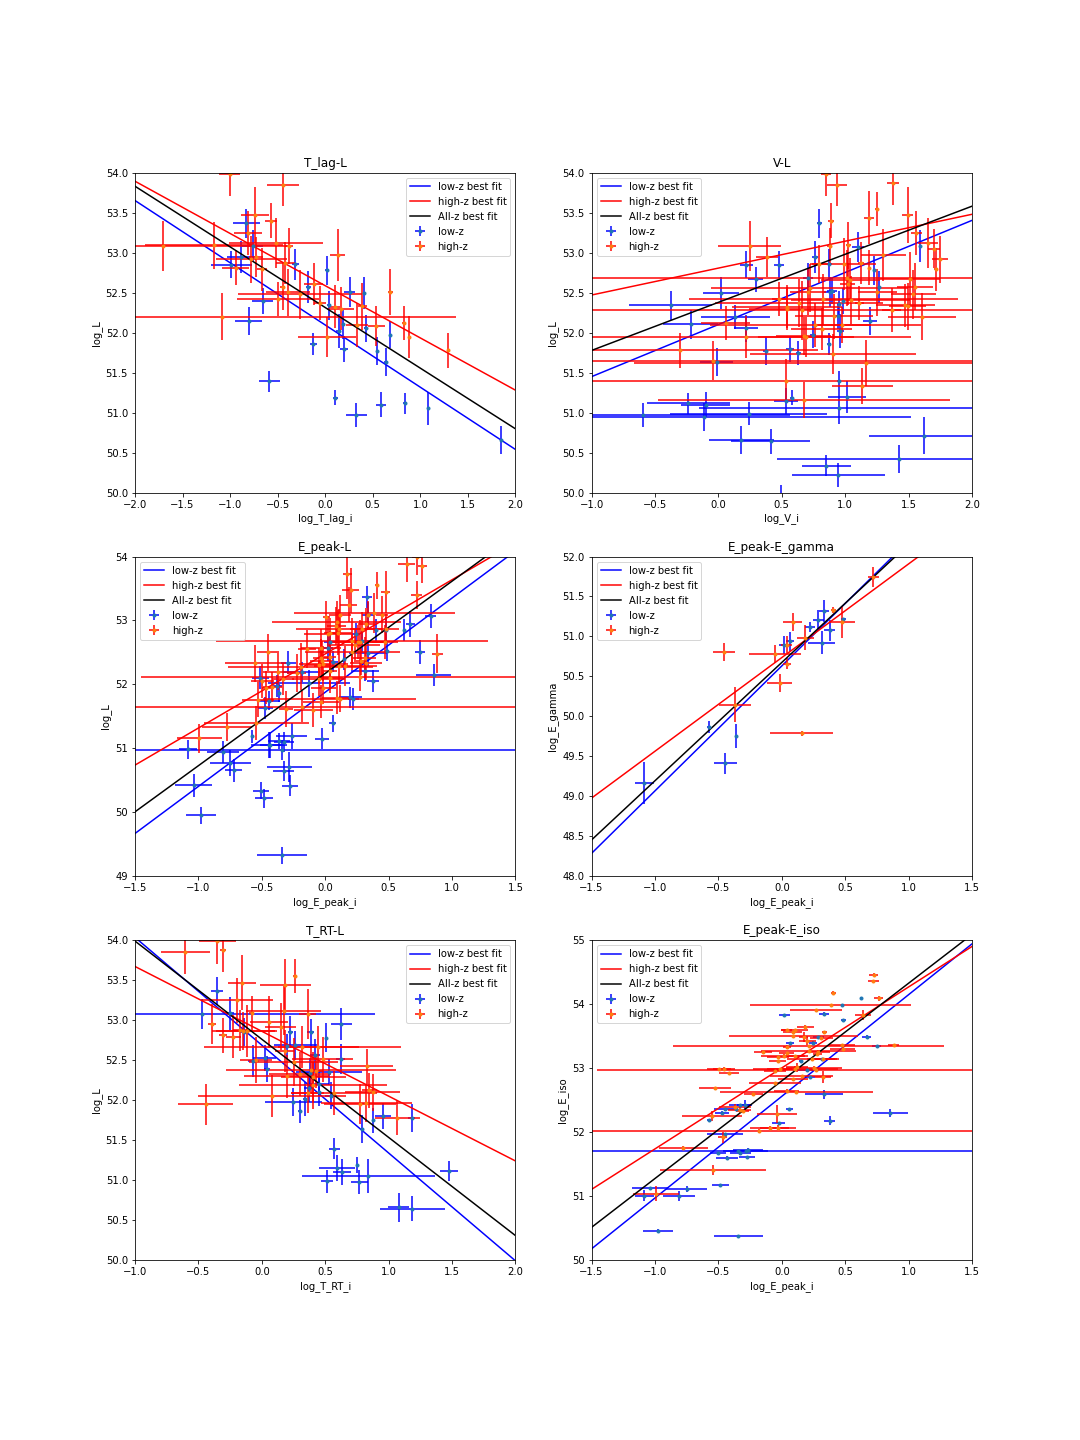
\includegraphics[width=\textwidth]{pantheon/gp/15_correlatin.png}
	\caption{Luminsosity correlations best fit}
	\label{fig:correlation_gp}
\end{figure}
